\epigraph{\textit{The business changes. The technology changes. The team changes. The team members change. The problem isn't change, per se, because change is going to happen; the problem, rather, is the inability to cope with change when it comes.}}{-- \textup{Kent Beck}}

During the early stages of the development, the first steps we followed were highly related to polishing and improving the solution described in the previous chapter. This was a challenging problem that resulted in a change in the project's direction, which will be detailed later.

\section{Technology stack}

As I mentioned earlier, the purpose of this second solution was to improve what was already implemented. This way, we kept most of the stack untouched. The sole change was the replacement of GraphX with its DataFrame equivalent library named GraphFrames.

\begin{figure}[ht]
    \centering
    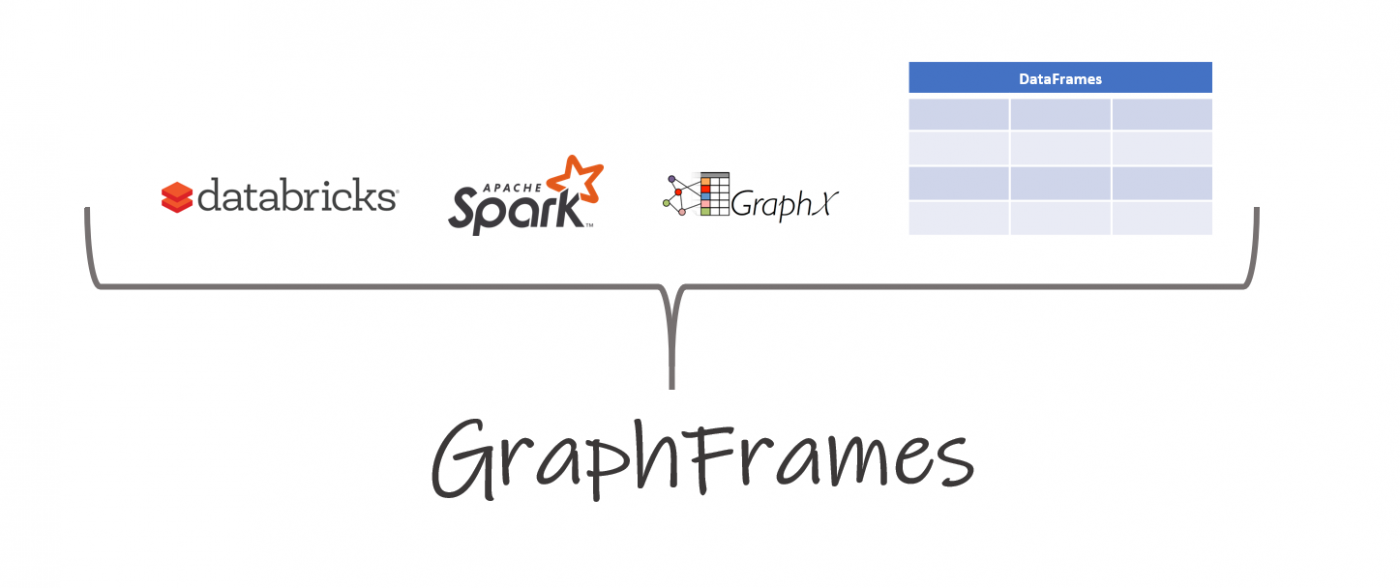
\includegraphics[width=.7\linewidth]{img/8-1_graphframes.png}
    \caption[Stack of the different technologies we are using for the second solution]{Stack of the different technologies we are using for the second solution\footnotemark}
\end{figure}

\footnotetext{\url{https://adatis.co.uk/graphframes/}}

\subsection{GraphFrames}

As it name goes, GraphFrame is a package for Apache Spark providing support for DataFrame-based Graphs. According to the introductory lines, the main goal of this stage of the development was to move our solution one step further in the abstraction level, from a solution based on RDDs to another based on DataFrames. From the ground up, we always believed RDDs weren't the go-to. What's more, RDDs are discouraged as they seem to be outdated in comparison to DataFrames and Datasets. More into this will be discussed in the next section. According to the description for GraphFrames, this API is similar to GraphX, except instead of being built on top of RDDs, they are built on DataFrames. The fact that the GraphFrames API for the Pregel algorithm has not been updated since 2018 makes us cautious of this approach.

\subsection{DataFrames and Datasets}

From Spark version 1.3 onwards, what were once known as SchemaRDDs are now referred to as DataFrames. That may give us an idea of what a DataFrame is. In that sense, they basically are RDDs provided some Schema for the data that is collected. With the help of this schema, DataFrames may be seen as rows with uniform structure: columns. Whereas RDDs are more akin to objects, DataFrames are closer to a table in a data base. This is quite relevant, as managing schemas to describe data allows us to perform operations over data in a much more efficient way than using Java serialization. It is worth mentioning that from Spark version 2.0 onwards, DataFrames can be understood as a type alias for \texttt{Dataset[Row]}, as they merged both APIs. In that sense, Datasets can be seen as the combination of the best from both worlds: with the appearance of a Java object from the outside, but with the shape of a table in RDBMS internally.

We now have a clear vision of what a DataFrame is. The problem is that even though they provide some nice features for data wrangling: schemas allow us to establish contracts so consumers know exactly the shape of the data they are working with, they are not so nicely implemented currently. Not only Apache Spark has no official support for working with DataFrame-based Graphs: notice GraphFrames is required, but the variety of supported types is scarce: including primitive types and Dates. Long has been discussed in this sense, but nothing has really changed since 2015\footnote{\url{https://issues.apache.org/jira/browse/SPARK-7768}}. To clarify this, let's put it into perspective.

\subsubsection{Encoders and User-defined Types}

% TODO: mention why Java serialization is so bad
% https://adtmag.com/articles/2018/05/30/java-serialization.aspx#:~:text=Serialization%20is%20brittle%2C%20it%20pokes,motivated%20getting%20it%20in%20there.

Working with simple data-structures is a trivial task in Apache Spark. What is not so easy to handle are custom data types. If the DataFrame cannot implicitly retrieve an Encoder, the user will be required to provide one. This is needed for Spark SQL to infer the schemas of the data we are working with. The complex the data-structure, the harder it is for the programmer to write an appropriate serialization/deserialization mechanism. Notice how this solution is far from efficient as it is based on serialization for data storage and retrieval, something we were trying to fix from the RDD-based solution. Another possibility could be writing your own User-defined type, which can be understood as a wrapper for the actual type. However, the amount of boiler-plate code needed, and the complexity of the data to be stored prevents us from writing an appropriate solution. More into this will be discussed in the following paragraphs.

% TODO: check what has been written here

As we have mentioned earlier, two main possible solutions arise for the problem of handling complex data: \textit{Custom encoders} and \textit{User-defined types}. It is a requirement for this solution not only to handle complex data, but unsupported, as we are not only trying to store complex data structures, but types that are not currently supported by the DataFrame API. This is a crucial argument against this DataFrame-based solution as we need to store URLs, which aren't supported by Spark SQL. The problem is that both of the mentioned solutions are inefficient. First, collection Encoders tend to act as bottlenecks in terms of performance. To follow up on this, storing non-standard objects in Spark is a mess\footnote{\url{https://stackoverflow.com/questions/36648128/how-to-store-custom-objects-in-dataset}}. The current situation of the Framework basically supports primitive types and not so complex case classes. The currently accepted solution in this sense consists of serializing objects using the \texttt{kryo} encoder which stores them as flat binary objects, preventing us from accessing concrete columns without deserializing the binary object. This last matter is specially crucial as messaging in Pregel is built on top of aggregates over particular columns. Hence, for each iteration we would need to serializing and deserialize every object stored. Thus, a custom, complex and inefficient encoder or type is not the solution we need. See figure \ref{fig:wikibaseClassDiagram} for an expanded description of the data model we are working with.

As a remark, it is worth noting that the code implementing the User-defined types for the data model above has a length of around 700 lines of code. While the actual algorithm takes around 100 lines of code to be written. For us to understand this, we have to describe how the so-called User-defined types are implemented in Apache Spark.

\begin{code}[User-defined types as implemented in Apache Spark]
    \inputminted{scala}{code/listings/8-1_udt.scala}
\end{code}

As noted in the first line of the above example, the description of user-defined types is annotated as an unstable API meant for developers. This implies that in minor Spark versions, the API may change or be eliminated. The use of it is at the user's own risk. As a consequence, if we follow this approach, we will end up with an unstable solution. Not only that but the processes for serializing and deserializing, along with the SQL schema -- which is no longer inferred by Scala's reflection system -- should be explicitly defined. Having said that, after we've specified what we've covered above, we're only establishing the wrapper, and yet no relationship is established between the real object and the User-defined type in the eyes of Spark's engine. To deal with this, we have two options: annotating the class we want to encapsulate or explicitly registering it. The former requires that the programmer has access to the class being wrapped. An ineffective technique that has been superseded by the latter since Spark 2.0. What's striking here is that it took Spark developers 6 years to come up with an answer in this regard. The API for user-defined types is essentially unmaintained, and dealing with custom objects in Spark is the framework's weak point. More on this was covered in the previously mentioned issue\footnote{\url{https://issues.apache.org/jira/browse/SPARK-7768}}.

\begin{code}[Registration of an User-defined type in Apache Spark]
    \inputminted{scala}{code/listings/8-2_udtRegistration.scala}
\end{code}

The issue here is the complexity of the data structures we use. According to the design in figure \ref{fig:wikibaseClassDiagram}, storing both \texttt{Statements} and \texttt{Entities} presents two major challenges. To begin, because the items stored require a fixed structure and we would like to polymorphically treat \texttt{Properties} and \texttt{Items} -- both -- as \texttt{Entities}, we need a mapping to convert from an object-oriented model to the relational paradigm. In this regard, we suggest \textit{Single Table Inheritance}\footnote{\url{https://en.wikipedia.org/wiki/Single_Table_Inheritance}}; that is, using a single table containing all the fields of all the child classes. The drawback is that we would end up with a solution in which rows contain redundant data: as many \texttt{NULL} values as different fields in child classes which are not the actual type for a certain row. Although it is a straightforward approach, it is inefficient. Second, this technique leads to a circular dependency\footnote{\url{https://en.wikipedia.org/wiki/Circular_dependency}} in which \texttt{Entities} include many \texttt{LocalStatements} that hold \texttt{Qualifiers} that may enclose \texttt{Entities}. When you define a schema for this problem, you eventually wind yourself in an infinite recursion where \texttt{Entities} have \texttt{Entities}. In conclusion, User-defined types offer a poor solution that causes several challenging issues.

\begin{figure}[ht]
    \centering
    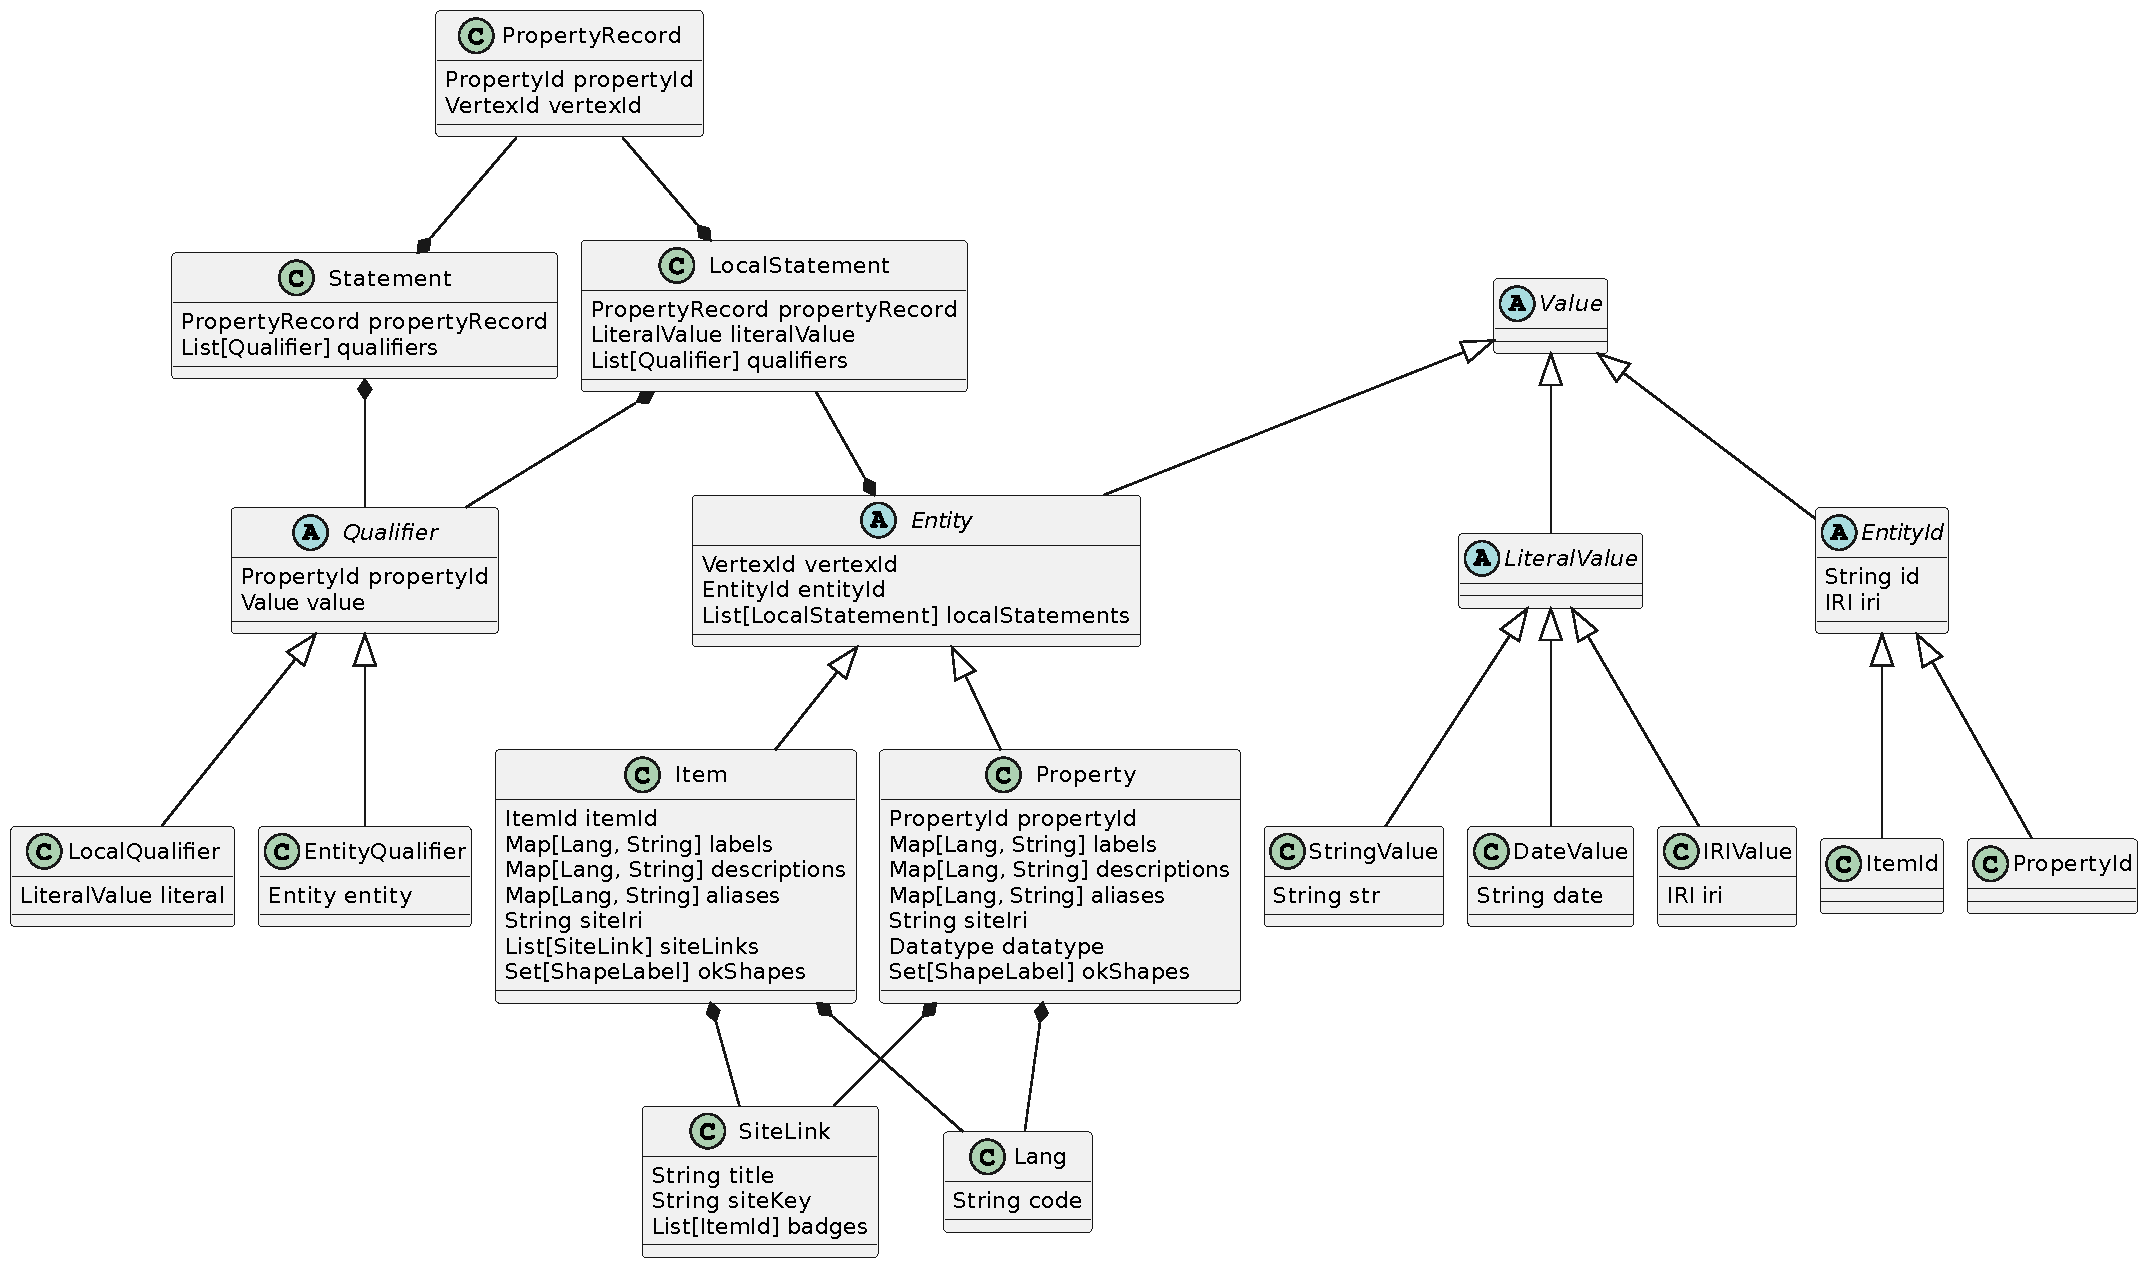
\includegraphics[width=\textwidth]{diagrams/8-1_wikibaseClassDiagram.pdf}
    \caption[Class diagram of the Wikibase data model as implemented in WShEx]{Class diagram of the Wikibase data model as implemented in WShEx\footnotemark}
    \label{fig:wikibaseClassDiagram}
\end{figure}
\footnotetext{\url{https://github.com/weso/shex-s}}